\chapter*{Appendix. \\ Self-supervised Learning trong bối cảnh Y khoa}

\addcontentsline{toc}{chapter}{Appendix. \\ Self-supervised Learning trong bối cảnh Y khoa}

\label{appendix:selfsl_medical}

\section{Động lực và bối cảnh}
\label{appendix:selfsl_motivation}

Trong lĩnh vực phân tích ảnh y khoa, việc huấn luyện các mô hình học sâu thường bị giới hạn nghiêm trọng bởi \textbf{sự thiếu hụt dữ liệu có nhãn chất lượng cao}. Quá trình gán nhãn yêu cầu sự tham gia của các chuyên gia lâm sàng, tiêu tốn nhiều thời gian, chi phí và dễ phát sinh sai khác giữa các chuyên gia (inter-observer variability). Điều này đặc biệt rõ rệt trong các bài toán như phát hiện tổn thương, phân đoạn khối u, hoặc xác định vùng bất thường trên ảnh y sinh.

Ngược lại, dữ liệu ảnh y khoa không nhãn lại tương đối dồi dào nhờ các hệ thống lưu trữ bệnh viện và quy trình chẩn đoán thường quy. Sự mất cân đối này đã thúc đẩy sự phát triển của các phương pháp học có khả năng tận dụng dữ liệu không nhãn một cách hiệu quả.

Trong bối cảnh đó, \textbf{\textit{Self-supervised Learning}} nổi lên như một hướng tiếp cận đặc biệt phù hợp. Không giống các phương pháp học có giám sát hoặc bán giám sát, Self-supervised Learning cho phép mô hình học biểu diễn trực tiếp từ dữ liệu không nhãn thông qua các nhiệm vụ tiền huấn luyện (pretext/proxy tasks), từ đó giảm đáng kể sự phụ thuộc vào nhãn thủ công và phù hợp với đặc thù của ảnh y khoa.

\subsection{Khái niệm cơ bản}
\label{appendix:selfsl_concepts}

Self-supervised Learning là một nhánh của học không giám sát, trong đó \textbf{tín hiệu giám sát được xây dựng trực tiếp từ chính dữ liệu}. Các phương pháp học trong thị giác máy tính có thể được phân biệt như sau:

\begin{itemize}
    \item \textbf{Supervised Learning}: sử dụng nhãn thủ công để tối ưu mô hình cho một nhiệm vụ cụ thể.
    \item \textbf{Unsupervised Learning}: học cấu trúc dữ liệu mà không có mục tiêu huấn luyện rõ ràng gắn với nhiệm vụ downstream.
    \item \textbf{Self-supervised Learning}: thiết kế các nhiệm vụ tiền huấn luyện có mục tiêu rõ ràng, trong đó nhãn được sinh tự động từ dữ liệu.
\end{itemize}

Trong Self-supervised Learning, mô hình thường được huấn luyện để học \textbf{biểu diễn đặc trưng (representation)} có khả năng tổng quát hóa, sau đó được sử dụng cho các bài toán downstream như phân loại, phát hiện hoặc phân đoạn. \\
Các phương pháp Self-supervised Learning thường dựa trên các giả định ngầm định sau:
\begin{itemize}
    \item dữ liệu chứa đủ thông tin cấu trúc để tạo tín hiệu học hữu ích,
    \item các biểu diễn tốt nên bất biến đối với các biến đổi không làm thay đổi ngữ nghĩa,
    \item việc học biểu diễn tổng quát giúp cải thiện hiệu năng trên nhiều nhiệm vụ y khoa khác nhau.
\end{itemize}

\subsection{Các nhóm phương pháp Self-supervised Learning}
\label{appendix:selfsl_methods}

Các phương pháp Self-supervised Learning trong thị giác máy tính và ảnh y khoa có thể được phân thành một số nhóm chính, phù hợp với các hướng tiếp cận được minh họa trong Hình~\ref{fig:selfsl_overview}:

\begin{itemize}
    \item \textbf{Pretext-task based methods (Innate relationship)}:
    thiết kế các nhiệm vụ nhân tạo như dự đoán phép biến đổi hình học (ví dụ: rotation prediction),
    sắp xếp mảnh ảnh (jigsaw puzzles) hoặc dự đoán vị trí tương đối để học biểu diễn.

    \item \textbf{Generative methods}:
    học biểu diễn thông qua các nhiệm vụ tái tạo dữ liệu đầu vào, điển hình là các mô hình autoencoder,
    trong đó encoder học biểu diễn và decoder học cách khôi phục ảnh ban đầu.

    \item \textbf{Contrastive learning}:
    học biểu diễn bằng cách kéo gần các cặp mẫu tương đồng (positive pairs) và đẩy xa các cặp không tương đồng,
    với các phương pháp tiêu biểu như SimCLR hoặc MoCo.

    \item \textbf{Self-prediction based methods}:
    yêu cầu mô hình dự đoán một phần thông tin bị che hoặc bị biến đổi từ phần còn lại của ảnh,
    bao gồm các phương pháp masked image modeling (ví dụ: MAE) và các chiến lược dự đoán đặc trưng.
\end{itemize}

\begin{figure}[H]
    \centering
    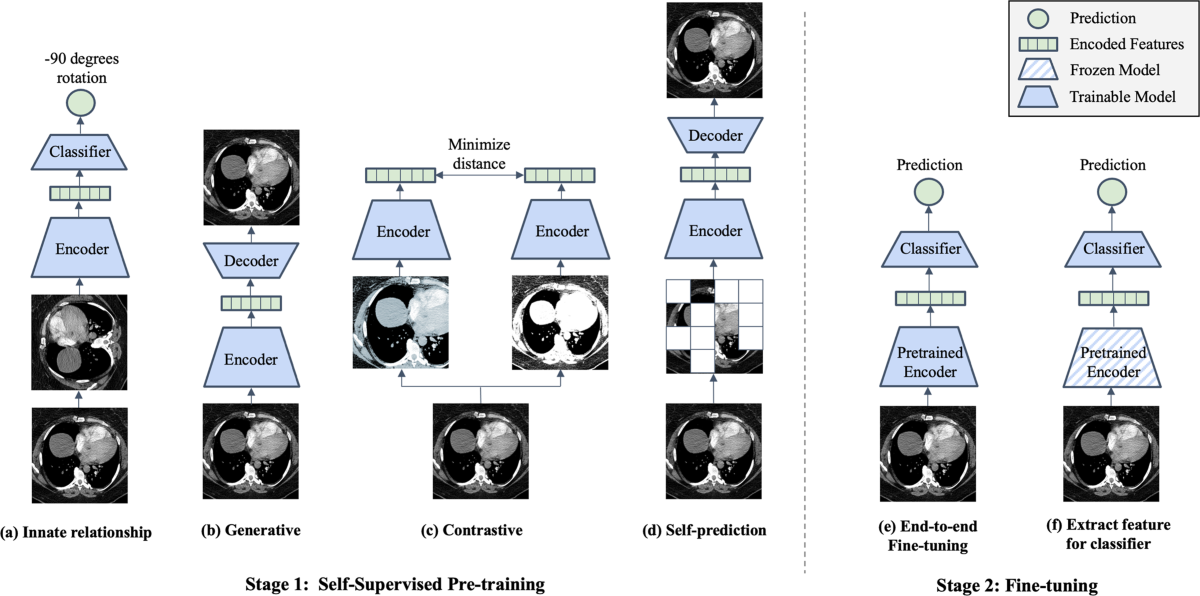
\includegraphics[width=1.0\linewidth]{img/appendix/self_supervised.png}
    \caption{Sơ đồ tổng quan của Self-supervised Learning trong thị giác máy tính:
    mô hình học biểu diễn từ dữ liệu không nhãn thông qua các nhiệm vụ tiền huấn luyện,
    sau đó được sử dụng cho các bài toán downstream trong ảnh y khoa.
    Hình minh họa được điều chỉnh từ các nghiên cứu tổng quan về self-supervised learning
    trong ảnh y khoa}
    \label{fig:selfsl_overview}
\end{figure}

Các nhóm phương pháp này đặc biệt phù hợp với ảnh y khoa, nơi việc học cấu trúc không gian và hình thái
đóng vai trò quan trọng hơn so với nhãn phân loại thuần túy, và dữ liệu không nhãn thường sẵn có với quy mô lớn.


\section{Liên hệ với bài toán Saliency và ROI}
\label{appendix:selfsl_saliency}

Trong ảnh y khoa, \textit{saliency maps} và \textit{Regions of Interest} (ROI) đóng vai trò quan trọng trong việc làm nổi bật các vùng có ý nghĩa lâm sàng. Trong bối cảnh Self-supervised Learning, các thông tin này có thể được tích hợp như một dạng \textbf{hướng dẫn yếu (weak guidance)} trong quá trình học biểu diễn.
Cụ thể, saliency hoặc ROI có thể được sử dụng để:
\begin{itemize}
    \item Định hướng các phép tăng cường dữ liệu nhằm tập trung vào vùng quan trọng,
    \item Giới hạn phạm vi học biểu diễn vào các cấu trúc liên quan về mặt y khoa,
    \item Cải thiện tính diễn giải của các biểu diễn học được.
\end{itemize}
Không giống các phương pháp dựa trên nhãn, việc kết hợp saliency và ROI trong Self-supervised Learning không yêu cầu nhãn chính xác ở mức pixel hoặc ảnh, mà chỉ đóng vai trò như một prior hình thái, phù hợp với điều kiện thực tế trong lâm sàng.

\begin{figure}[H]
  \centering
  \begin{subfigure}{\linewidth}
    \centering
    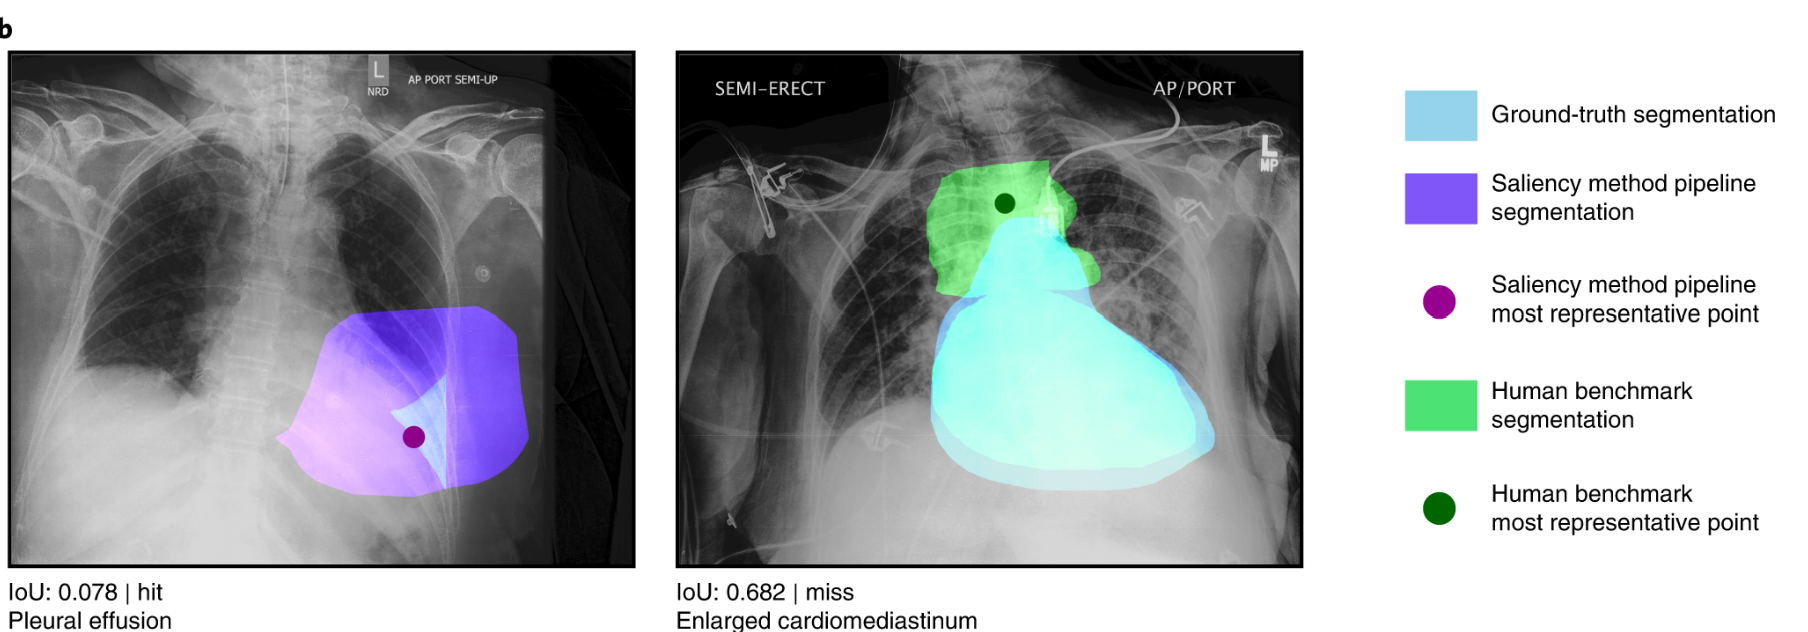
\includegraphics[width=0.75\linewidth]{img/appendix/saliency_roi.png}
    \caption{}
  \end{subfigure}

  \vspace{0.5em}

  \begin{subfigure}{\linewidth}
    \centering
    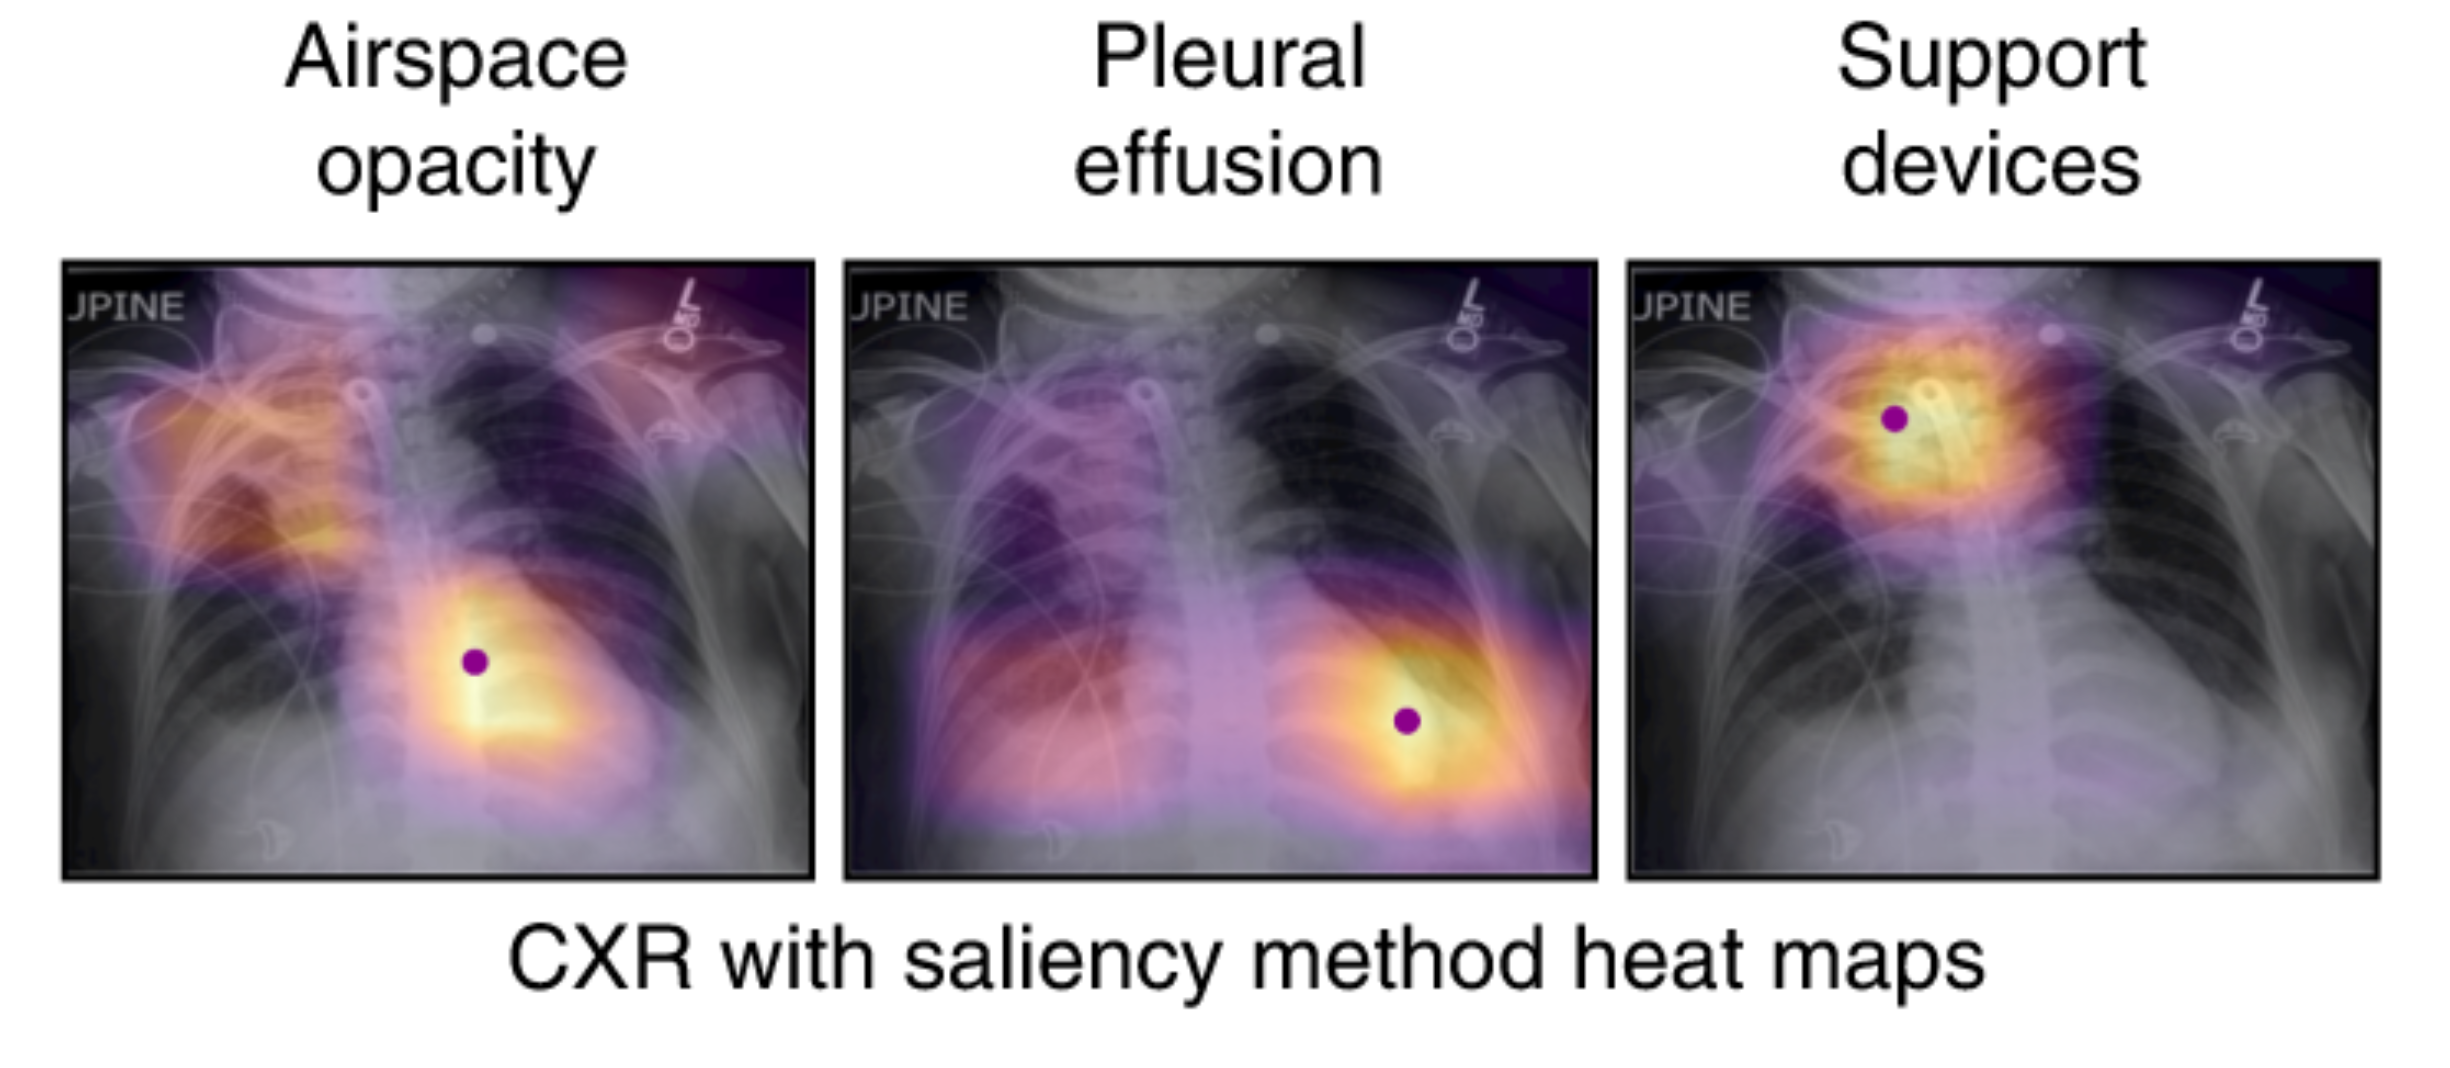
\includegraphics[width=0.75\linewidth]{img/appendix/saliency_roi2.png}
    \caption{}
  \end{subfigure}

  \caption{Minh họa vai trò của saliency map và ROI như thông tin hướng dẫn yếu
  trong Self-supervised Learning cho ảnh y khoa.
  (a) Saliency heatmaps chồng lên ảnh X-quang ngực cho các nhãn bệnh khác nhau.
  (b) Các vùng ROI suy ra từ saliency và so sánh với phân đoạn chuẩn và phân đoạn
  từ chuyên gia, cho thấy saliency map có thể cung cấp thông tin không gian
  mang ý nghĩa lâm sàng mà không cần nhãn phân đoạn chính xác.}
  \label{fig:selfsl_saliency_roi}
\end{figure}


\section{Rủi ro và hạn chế của Self-supervised Learning}
\label{appendix:selfsl_risks}

Mặc dù Self-supervised Learning mang lại nhiều lợi ích trong phân tích ảnh y khoa,
các phương pháp này vẫn tồn tại một số rủi ro và hạn chế cần được xem xét.

\begin{itemize}
    \item \textbf{Phụ thuộc vào nhiệm vụ tiền huấn luyện}:
    hiệu quả của mô hình phụ thuộc mạnh vào thiết kế pretext task;
    các nhiệm vụ không phù hợp có thể dẫn đến việc học các đặc trưng
    kém liên quan đến bài toán downstream.

    \item \textbf{Nguy cơ học đặc trưng không mang ý nghĩa lâm sàng}:
    trong điều kiện không có nhãn, mô hình có thể tập trung vào
    các mẫu thống kê bề mặt thay vì các cấu trúc bệnh lý quan trọng.

    \item \textbf{Độ nhạy với phép tăng cường dữ liệu}:
    các phép biến đổi không phù hợp với đặc thù ảnh y khoa
    có thể làm suy giảm chất lượng biểu diễn học được.

    \item \textbf{Chi phí tính toán và khả năng triển khai}:
    giai đoạn tiền huấn luyện thường yêu cầu dữ liệu lớn
    và tài nguyên tính toán đáng kể.

    \item \textbf{Khoảng cách giữa tiền huấn luyện và nhiệm vụ downstream}:
    biểu diễn học được không phải lúc nào cũng tối ưu
    cho mọi bài toán lâm sàng cụ thể.
\end{itemize}

Các rủi ro này được minh họa trong Hình~\ref{fig:selfsl_risk_saliency} và Hình~\ref{fig:selfsl_risk_augmentation}, cho thấy mô hình self-supervised
có thể tập trung sai vùng quan trọng hoặc bị ảnh hưởng bởi các phép tăng cường
dữ liệu không phù hợp với đặc thù ảnh y khoa.

\begin{figure}[H]
  \centering
  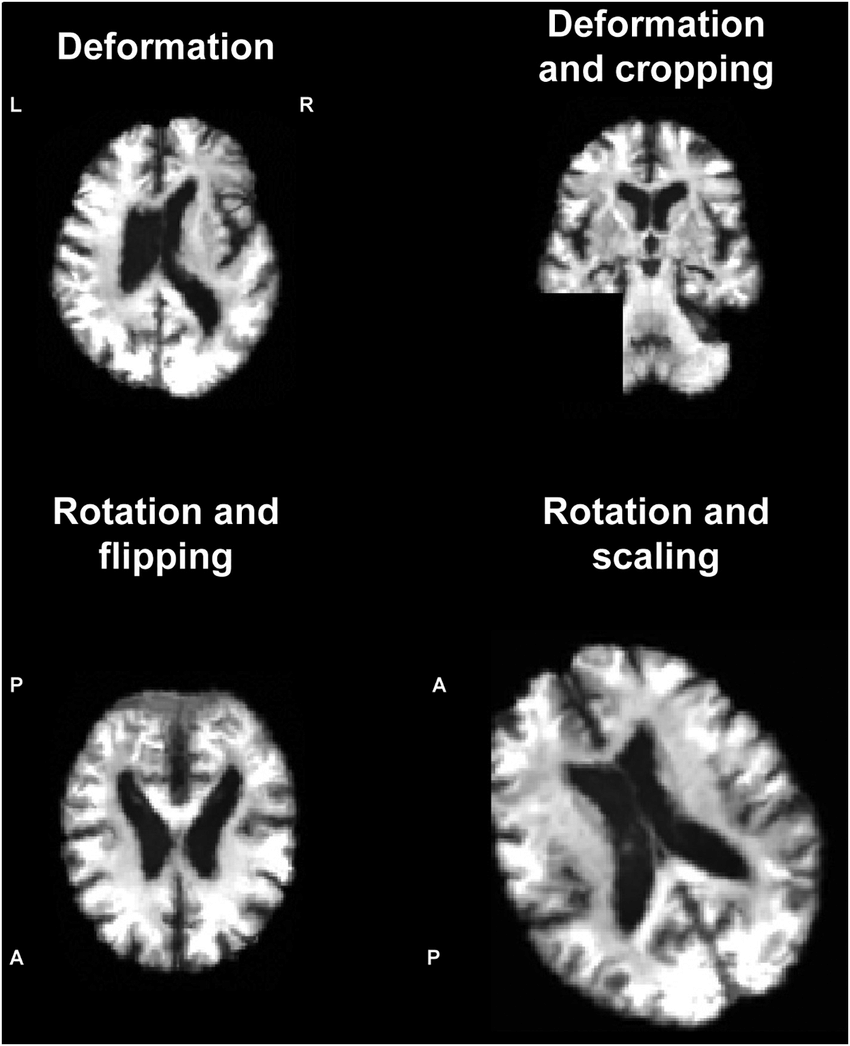
\includegraphics[width=0.4\linewidth]{img/appendix/fail_after_augmentation.png}
  \caption{Ví dụ minh họa ảnh hưởng của các phép tăng cường dữ liệu mạnh trong Self-supervised Learning,
  trong đó các biến đổi hình học như deformation, cropping hoặc scaling
  có thể làm thay đổi cấu trúc giải phẫu.
  Hình ảnh được điều chỉnh từ các nghiên cứu về data augmentation trong ảnh y khoa}
  \label{fig:selfsl_risk_augmentation}
\end{figure}

\begin{figure}[H]
  \centering
  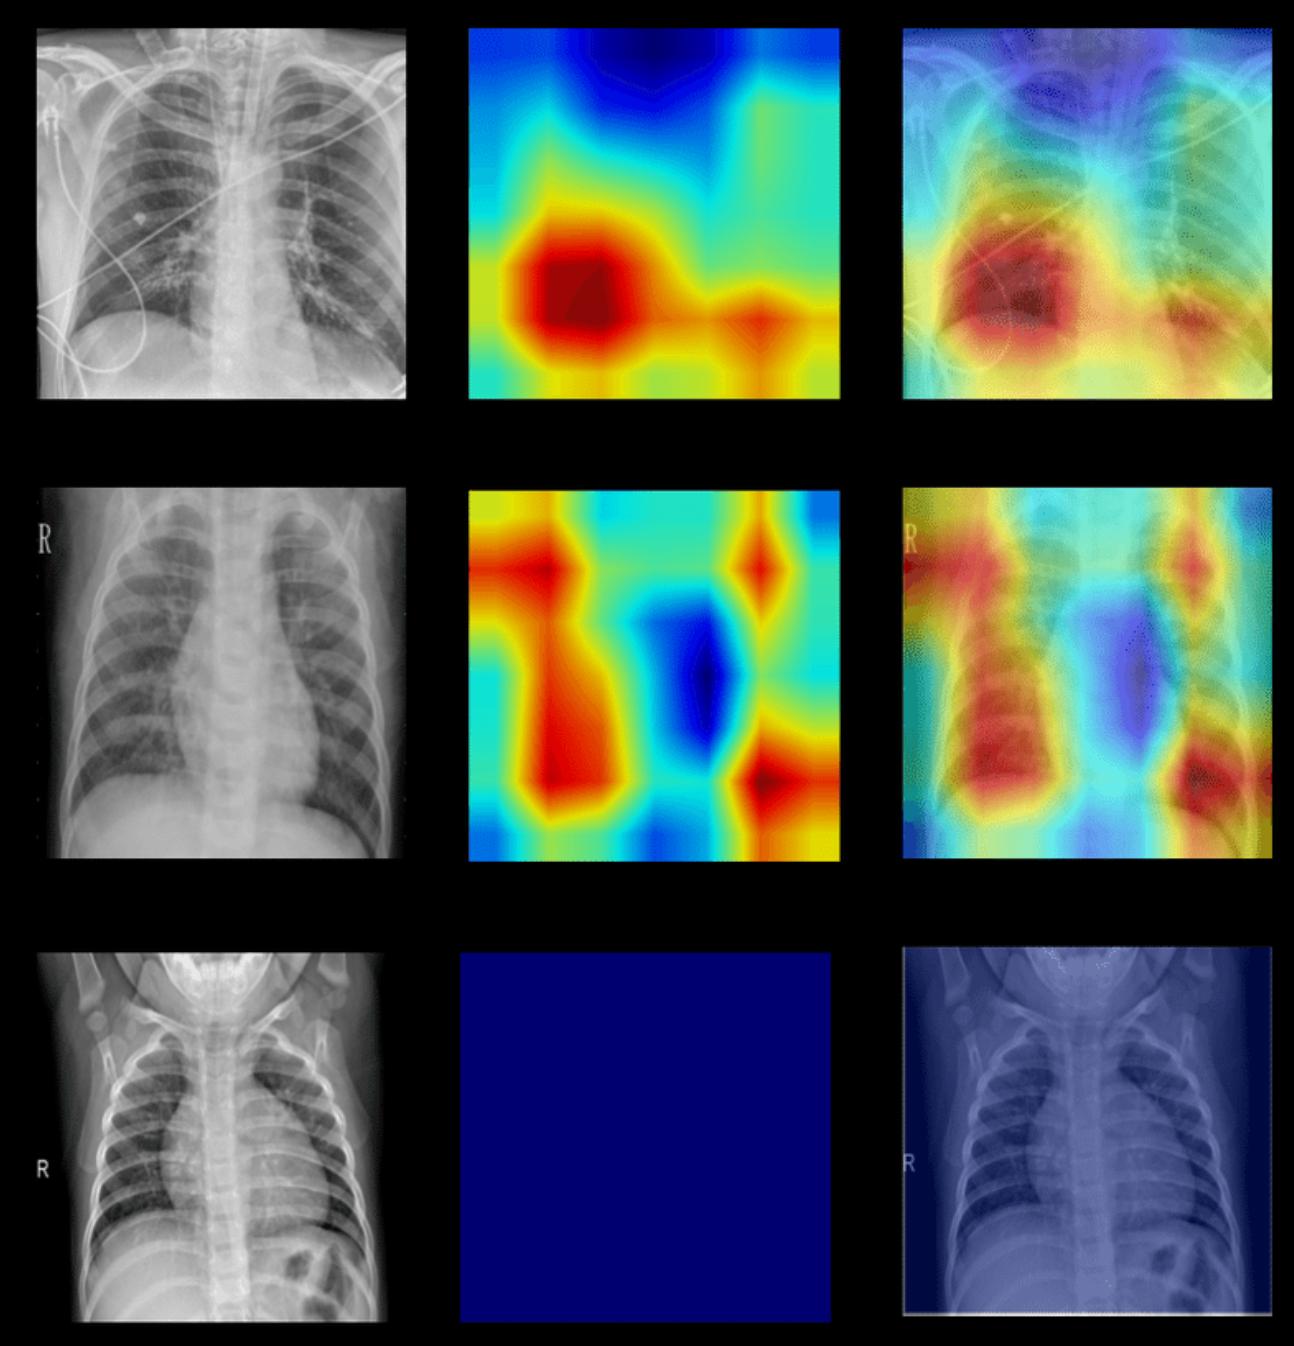
\includegraphics[width=0.4\linewidth]{img/appendix/fail_saliency.png}
  \caption{Ví dụ minh họa một rủi ro của Self-supervised Learning trong ảnh y khoa,
   trong đó saliency map của mô hình tập trung vào các vùng không mang ý nghĩa lâm sàng.
   Hình ảnh được điều chỉnh từ các nghiên cứu về khả năng diễn giải và phân tích sai lệch
   của mô hình học sâu trong ảnh X-quang.}
  \label{fig:selfsl_risk_saliency}
\end{figure}

\section{Thực nghiệm với mô hình SSiT}

Trong phần mở rộng này, chúng em tiến hành thử nghiệm mô hình SSiT (Saliency-guided Self-supervised Image Transformer) nhằm kiểm tra khả năng sử dụng bản đồ saliency như một tín hiệu dẫn hướng trong bài toán học tự giám sát cho ảnh võng mạc. Mục tiêu chính của phần thực nghiệm này không phải là xây dựng một hệ thống hoàn chỉnh ở mức nghiên cứu khoa học, mà là kiểm chứng tính khả thi của việc kết hợp saliency map truyền thống với mô hình học biểu diễn hiện đại.

\begin{figure}
  \centering
  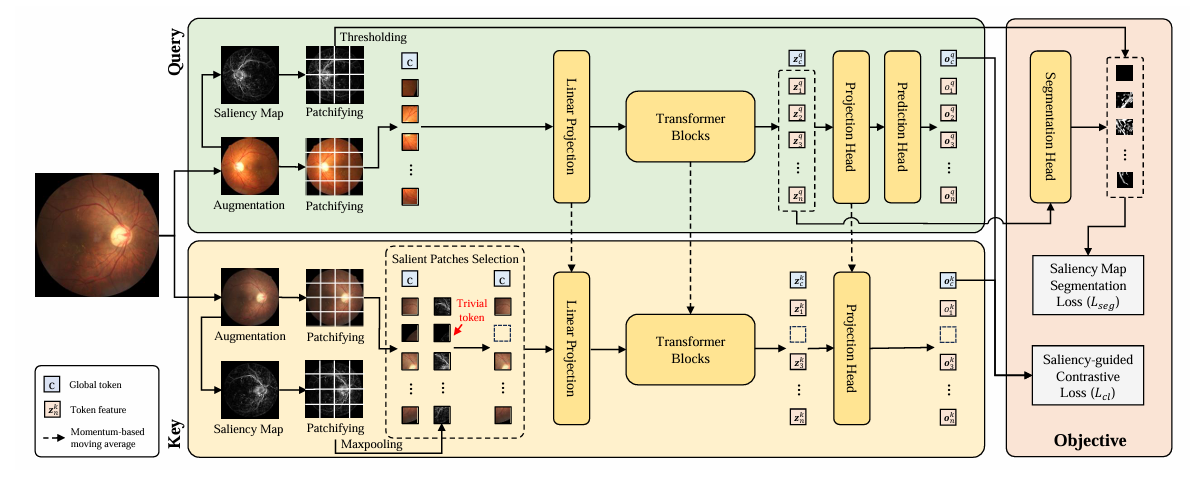
\includegraphics[width=0.8\linewidth]{img/appendix/frame-work.PNG}
  \caption{Sơ đồ tổng quan mô hình SSiT:
  sử dụng saliency map như tín hiệu dẫn hướng trong quá trình học tự giám sát
  nhằm tập trung vào các vùng quan trọng về mặt lâm sàng trong ảnh võng mạc.
  Hình minh họa được điều chỉnh từ bài báo gốc của SSiT}
  \label{fig:selfsl_ssit_overview}
\end{figure}

\subsection{Mô tả tập dữ liệu}

\subsubsection{Tập dữ liệu tiền huấn luyện (Pre-training)}

Trong giai đoạn học tự giám sát, chúng em sử dụng tập dữ liệu DRIONS-DB (như phần thực nghiệm ở Chương 4) đã được tiền xử lý và sinh saliency map ở các chương trước. Mỗi mẫu dữ liệu bao gồm:
\begin{itemize}
    \item Ảnh đáy mắt gốc (không nhãn phân loại hoặc phân vùng),
    \item Bản đồ saliency tương ứng, được sinh bằng các phương pháp truyền thống (Center-Surround).
\end{itemize}

\begin{figure}[H]
  \centering
  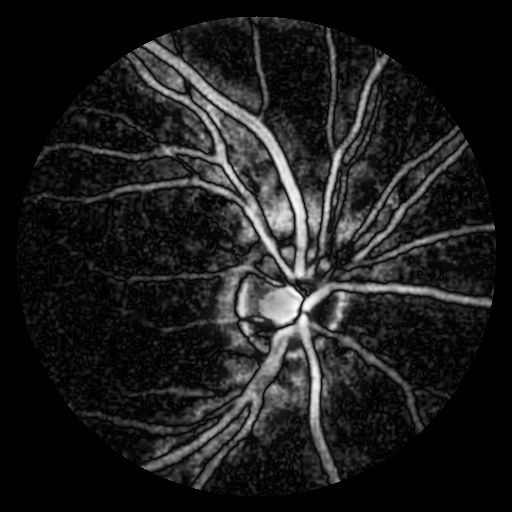
\includegraphics[width=0.6\linewidth]{img/appendix/saliency_cs.jpg}
  \caption{Minh họa một số mẫu ảnh và bản đồ saliency từ tập dữ liệu DRIONS-DB}
  \label{fig:selfsl_drionsdb_samples}
\end{figure}

Tập dữ liệu này có quy mô nhỏ (110 ảnh), phù hợp với bối cảnh đồ án môn học, đồng thời phản ánh đúng khó khăn thực tế của ảnh y khoa là thiếu dữ liệu gán nhãn.

\subsubsection{Tập dữ liệu downstream}

Để đánh giá gián tiếp chất lượng biểu diễn học được, mô hình sau tiền huấn luyện được kiểm tra trên các bài toán downstream tiêu biểu trong nhãn khoa, bao gồm:
DDR, APTOS 2019, Messidor-2 (phân loại) và DRIVE, IDRiD (phân vùng)
\href{https://www.kaggle.com/datasets/ascanipek/eyepacs-aptos-messidor-diabetic-retinopathy}{\texttt{dataset links (Kaggle)}}

. Trong phạm vi đồ án, các thí nghiệm downstream chủ yếu được sử dụng để quan sát xu hướng và khả năng tổng quát hóa, chưa tập trung tối ưu chi tiết từng tập dữ liệu.

\subsection{Quy trình học tự giám sát}

SSiT được xây dựng trên kiến trúc Vision Transformer (ViT), trong đó saliency map được tích hợp trực tiếp vào quá trình học tự giám sát nhằm hướng mô hình tập trung vào các vùng quan trọng về mặt lâm sàng.

Trong quá trình tiền huấn luyện, mỗi ảnh đầu vào được kết hợp với bản đồ saliency tương ứng để điều chỉnh các phép biến đổi dữ liệu và cơ chế attention. Cách tiếp cận này giúp mô hình giảm sự chú ý vào các vùng nền không liên quan và tập trung nhiều hơn vào các cấu trúc quan trọng như đĩa thị hoặc tổn thương.

\subsection{Hàm mất mát (Loss Function)}

Trong mô hình SSiT, quá trình học tự giám sát được điều khiển thông qua hai thành phần hàm mất mát chính, trong đó bản đồ saliency đóng vai trò như một tín hiệu dẫn hướng không gian. Giả sử ảnh đầu vào là $I$, bản đồ saliency tương ứng là $S$, và mô hình Transformer sinh ra biểu diễn đặc trưng $z = f_\theta(I)$.

\paragraph{Saliency-guided Contrastive Loss}
Mục tiêu của thành phần này là học các biểu diễn sao cho các vùng có giá trị saliency cao được ánh xạ gần nhau trong không gian đặc trưng, đồng thời giảm ảnh hưởng của các vùng nền hoặc nhiễu. 

Cụ thể, saliency map $S$ được sử dụng để gán trọng số cho các patch hoặc token trong ảnh. Với hai mẫu tăng cường khác nhau của cùng một ảnh, ký hiệu là $I^{(1)}$ và $I^{(2)}$, hàm mất mát tương phản được xây dựng dưới dạng:
\[
\mathcal{L}_{\text{SC}} = 
- \sum_{i} w_i \log 
\frac{\exp(\mathrm{sim}(z_i^{(1)}, z_i^{(2)}) / \tau)}
{\sum_{j} \exp(\mathrm{sim}(z_i^{(1)}, z_j^{(2)}) / \tau)},
\]
trong đó $z_i^{(1)}, z_i^{(2)}$ là các đặc trưng tương ứng của patch $i$, $\mathrm{sim}(\cdot,\cdot)$ là hàm đo độ tương đồng (ví dụ cosine similarity), $\tau$ là tham số nhiệt độ, và $w_i$ là trọng số saliency thu được từ $S$. Nhờ đó, các patch quan trọng về mặt không gian được ưu tiên trong quá trình học biểu diễn.

\paragraph{Saliency Segmentation Loss}
Thành phần Saliency Segmentation Loss sử dụng bản đồ saliency như một dạng nhãn yếu (weak supervision) nhằm duy trì thông tin không gian ở các vùng quan trọng. Giả sử $\hat{S}$ là bản đồ chú ý hoặc bản đồ dự đoán nội bộ của mô hình, hàm mất mát được định nghĩa dưới dạng:
\[
\mathcal{L}_{\text{SS}} = \frac{1}{|\Omega|} \sum_{(x,y) \in \Omega}
\left\| \hat{S}(x,y) - S(x,y) \right\|^2,
\]
trong đó $\Omega$ là miền ảnh. Thành phần này buộc mô hình duy trì sự tương thích giữa vùng chú ý học được và vùng có saliency cao, từ đó hạn chế việc mất chi tiết khi áp dụng các phép biến đổi dữ liệu mạnh.

\paragraph{Hàm mất mát tổng}
Tổng hàm mất mát của mô hình SSiT được xây dựng dưới dạng tổ hợp tuyến tính có trọng số của hai thành phần trên:
\[
\mathcal{L} = \lambda_1 \mathcal{L}_{\text{SC}} + \lambda_2 \mathcal{L}_{\text{SS}},
\]
trong đó $\lambda_1$ và $\lambda_2$ là các hệ số điều chỉnh nhằm cân bằng giữa việc học biểu diễn toàn cục và việc bảo toàn thông tin không gian cục bộ. Việc lựa chọn các hệ số này được thực hiện thực nghiệm và phù hợp với quy mô nhỏ của tập dữ liệu trong đồ án.

\subsection{Chiến lược huấn luyện và validation}

Do tập dữ liệu tiền huấn luyện có quy mô nhỏ, chúng em sử dụng cấu hình huấn luyện đơn giản với số epoch vừa phải và learning rate thấp để tránh hiện tượng quá khớp. Quá trình huấn luyện được thực hiện trên môi trường Kaggle với GPU đơn hoặc đa GPU tùy điều kiện tài nguyên.

Việc đánh giá (validation) trong giai đoạn tự giám sát không dựa trên nhãn ground truth, mà chủ yếu thông qua:
\begin{itemize}
    \item Quan sát độ ổn định của loss trong quá trình huấn luyện,
    \item Đánh giá định tính bản đồ attention và vùng mô hình tập trung,
    \item Hiệu quả của mô hình khi fine-tuning trên các bài toán downstream.
\end{itemize}

\subsection{Nhận xét và đánh giá}

Kết quả thực nghiệm cho thấy việc tích hợp saliency map vào mô hình SSiT giúp mô hình học biểu diễn có định hướng hơn so với học tự giám sát thuần túy. Đặc biệt, trong bối cảnh dữ liệu nhỏ và không có nhãn, saliency đóng vai trò như một tín hiệu dẫn hướng hữu ích, giúp mô hình tập trung vào các vùng mang ý nghĩa lâm sàng.

\begin{figure}
  \centering
  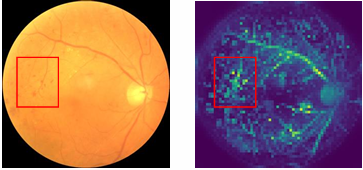
\includegraphics[width=0.6\linewidth]{img/appendix/ssiT.PNG}
  \caption{Minh họa bản đồ attention học được từ mô hình SSiT,
  cho thấy mô hình tập trung vào các vùng quan trọng như đĩa thị và mạch máu
  trong ảnh võng mạc.}
  \label{fig:selfsl_ssit_attention}
\end{figure}

Tuy nhiên, do quy mô dữ liệu và phạm vi đồ án còn hạn chế, chúng em chưa thể đánh giá đầy đủ hiệu quả của SSiT ở mức độ định lượng sâu. Việc lựa chọn trọng số giữa các thành phần loss và chiến lược validation cũng chưa được tối ưu toàn diện.

Nhìn chung, phần thực nghiệm này cho thấy tiềm năng của việc kết hợp saliency map truyền thống với các mô hình học tự giám sát hiện đại. Đây là một hướng tiếp cận phù hợp để mở rộng trong các nghiên cứu hoặc đồ án chuyên sâu hơn trong tương lai.


